%% Road-collision severity ablation: research paper (IEEE conference format, US letter).
%% Build:   ./build.sh  (compiles on the GPU server: pdflatex, bibtex, pdflatex x2)
%% Figures: python scripts/14_paper_figures.py --out paper/figures   (run from the project root)
\documentclass[conference,letterpaper]{IEEEtran}
\IEEEoverridecommandlockouts

\usepackage{cite}
\usepackage{amsmath,amssymb,amsfonts}
\usepackage{graphicx}
\usepackage{textcomp}
\usepackage{xcolor}
\usepackage{booktabs}
\usepackage{multirow}
\usepackage{array}
\usepackage{url}
\usepackage{tikz}
\usetikzlibrary{arrows.meta,positioning,calc}
\usepackage[hidelinks]{hyperref}

\definecolor{fitc}{HTML}{3F7FD0}
\definecolor{tunec}{HTML}{2E9E78}
\definecolor{calc}{HTML}{25466F}
\definecolor{testc}{HTML}{D9653B}

\begin{document}

\title{Feature Engineering, Imbalance Handling and Calibration for Crash-Severity Prediction: An Out-of-Time Ablation on STATS19}

\author{\IEEEauthorblockN{1\textsuperscript{st} Tahir Ahmed Khan}
\IEEEauthorblockA{25I-8025\\
MS Data Science\\
Islamabad, Pakistan\\
Email: i258025@isb.nu.edu.pk}
\and
\IEEEauthorblockN{2\textsuperscript{nd} Ahmed Qamar}
\IEEEauthorblockA{25I-8049\\
MS Data Science\\
Islamabad, Pakistan\\
Email: i258049@isb.nu.edu.pk}
\and
\IEEEauthorblockN{3\textsuperscript{rd} Ali Raza}
\IEEEauthorblockA{25I-8043\\
MS Data Science\\
Islamabad, Pakistan\\
Email: i258043@isb.nu.edu.pk}}

\maketitle

\begin{abstract}
Recent crash-severity studies combine several techniques in one pipeline, so the contribution of each technique, and its performance on later data, is hard to assess. We ran a controlled ablation on 306,710 police-reported collisions from the UK STATS19 database (2023--2025). Feature engineering with selection, cost-sensitive learning (class weighting, random undersampling and SMOTE-NC) and post-hoc calibration were varied independently across six model families. Models were trained on 2023 and half of 2024, calibrated and thresholded on the other half of 2024, and scored on 2025 under a frozen, hash-checked protocol. The selected LightGBM model reached an average precision (PR-AUC) of 0.496 against a no-skill value of 0.262, and an ROC-AUC of 0.730. Engineered features raised PR-AUC significantly for logistic regression, a decision tree, random forest and XGBoost (+0.004 to +0.017), but not for LightGBM or CatBoost. Class weighting raised recall at the default 0.5 threshold by 0.47 to 0.52, yet no significant $F_2$ difference was detected once each arm had its own tuned threshold, and SMOTE-NC lowered PR-AUC in all six configurations where it was tested. Calibration reduced the expected calibration error of weighted or undersampled models from about 0.2 to about 0.01. Under an assumed 5:1 cost of missed severe collisions to false alarms, the Bayes threshold of 1/6 on calibrated scores raised the recall of the final model from 0.21 to 0.86 and lowered expected cost by 43\%; for this unweighted model almost all of that gain came from the threshold.
\end{abstract}

\begin{IEEEkeywords}
Road safety, crash severity, class imbalance, cost-sensitive learning, probability calibration, decision threshold, temporal validation, STATS19
\end{IEEEkeywords}

%% ======================================================================
\section{Introduction}

About one in four injury collisions reported to the police in Great Britain is severe, meaning that at least one person was killed or seriously injured. A model that estimates this outcome from the circumstances of a collision, such as place, time, road, weather and the road users involved, could help to rank incidents and to show which conditions are associated with serious harm. The task is a binary classification problem with an imbalanced target, non-linear effects and, for flexible models, probabilities that may not be calibrated.

Recent studies on this problem combine different subsets of feature engineering, resampling or class weighting, gradient boosting, calibration, threshold tuning and SHAP explanations~\cite{le2026ksi,alhawarat2026calibrated,gao2026ensemble}. When several of these steps change together, their separate contributions cannot be read off the results. The evaluation design also differs: of the two closest STATS19 studies, one used a random split of the same years~\cite{le2026ksi} and the other trained on earlier years and tested on a later one~\cite{alhawarat2026calibrated}. Testing on a later year is closer to how such a model would be used.

We do not propose a new classifier. Instead, we measure how much three common techniques add to severe-collision detection on STATS19 data for 2023--2025~\cite{dft2026stats19}, using a later year as the test set. The research questions are:
\begin{itemize}
\item \textbf{RQ1:} How much do engineered and selected features improve severe-collision classification over the raw feature set on a later year?
\item \textbf{RQ2:} How much does cost-sensitive learning (class weighting or resampling) improve detection of the severe class when features and calibration are held fixed?
\item \textbf{RQ3:} Does post-hoc calibration, together with threshold selection, improve the reliability of the predictions on a later year?
\end{itemize}
The study combines a column-level audit of usable fields, an ablation with 144 fitted models and 18 primary contrasts fixed before the test year was scored.

%% ======================================================================
\section{Literature Review}

Le~\cite{le2026ksi} modelled killed-or-seriously-injured (KSI) collisions in STATS19 for 2020--2024 with LightGBM. The study compared SMOTE with class weighting, tuned the threshold, calibrated the output and used SHAP, and it evaluated on a stratified random 80/20 split. LightGBM reached an ROC-AUC of 0.664 with SMOTE and 0.692 with class weighting, and the weighted model had the highest recall but the worst Brier score. Alhawarat \textit{et al.}~\cite{alhawarat2026calibrated} trained gradient-boosting models on STATS19 for 2016--2020, calibrated on 2021 and tested on 2022. Their LightGBM model retrained on UK data reached an ROC-AUC of 0.651 and a PR-AUC of 0.369. Neither study varies each technique separately across several model families, which is the focus of our work.

Other studies use ensembles and post-hoc explanation. Gao \textit{et al.}~\cite{gao2026ensemble} combined XGBoost, random forest, CatBoost and LightGBM by soft voting and explained them with SHAP and accumulated local effects, using road-geometry variables that STATS19 does not contain. Xiao and Duan~\cite{xiao2025multitask} proposed an explainable multi-task deep network on multi-source data from China. Interpretable models have also been applied to US national data~\cite{abdulrashid2025interpretable}, to expressway crashes in Sri Lanka~\cite{madushani2023expressway} and to motorcycle crashes in Pakistan~\cite{mansoor2023motorcycle}.

For class imbalance, Chen \textit{et al.}~\cite{chen2025imbalanced} compared combinations of resampling methods and classifiers on imbalanced crash data, and Mostafa \textit{et al.}~\cite{mostafa2025ai} combined feature engineering, clustering, oversampling and feature selection. SMOTE~\cite{chawla2002smote} creates synthetic minority examples by interpolating between neighbours. A different route changes the decision rule instead of the data: Elkan~\cite{elkan2001foundations} showed that, with calibrated probabilities, the cost-optimal decision is a threshold fixed by the cost ratio, and that under his assumptions changing the class proportions in training has the same effect as moving that threshold. Platt scaling~\cite{platt1999probabilistic} and isotonic regression~\cite{zadrozny2002transforming} are standard post-hoc calibrators, and the expected calibration error (ECE) is a common summary of miscalibration~\cite{guo2017calibration}. Islam \textit{et al.}~\cite{islam2024calibrated} applied calibrated confidence learning to real-time crash and severity prediction, and two recent systematic reviews survey machine-learning crash prediction and its open problems~\cite{chai2024review,ali2024review}.

%% ======================================================================
\section{Proposed Methodology}

\subsection{Data and Availability Rule}

We used the final STATS19 releases for 2023, 2024 and 2025~\cite{dft2026stats19}. Each year has a collision table (44 columns), a vehicle table (32) and a casualty table (24), linked by a collision identifier, giving 306,710 collisions, 557,277 vehicle records and 389,132 casualty records. Codes were decoded with the 2025 data guide, and codes introduced in 2024 without a 2023 equivalent (journey purpose 8 and 9, manoeuvre 20) were set to missing. The target is $y=1$ (severe) for fatal or serious collisions and $y=0$ for slight ones. Fatal collisions are about 1.5\% of the total, so the severe class is mostly serious collisions.

The data are retrospective police records, so we applied an assumed availability rule: a field may be used only if it describes the circumstances before impact (place, time, road, environment, vehicles, drivers and manoeuvres) rather than the outcome, the impact sequence or police processing. Each of the 100 raw columns was given one decision in a registry checked by unit tests: 41 kept, 14 dropped as leakage, 26 dropped as redundant or superseded, 12 dropped as identifiers, five crash-mechanics fields held out for a sensitivity analysis, one target and one field used only for evaluation. The leakage group includes the number of casualties, casualty severity and DfT's severity-adjustment columns. Police attendance was used only for evaluation, because it is strongly associated with severity (in 2023--2024, 30.2\% of attended collisions were severe, against 9.7\% of self-reported ones). Four pedestrian fields come from the casualty table, so they describe an injured pedestrian (the one with the lowest casualty reference); their effect is tested in Section~\ref{sec:sens}. Vehicle records were summarised per collision without depending on vehicle order: counts per code, and the minimum, mean and maximum of driver age and engine size.

\subsection{Temporal Design and Frozen Protocol}

Table~\ref{tab:splits} and Fig.~\ref{fig:design} show the splits. FIT (2023) is used to fit models, encoders, feature selection and resampling. TUNE (2024, odd ISO weeks) is used for early stopping and hyper-parameter search, and CAL (2024, even ISO weeks) only for calibrators, thresholds and model selection. Alternating weeks give TUNE and CAL the same seasonal coverage. After tuning, each configuration was refitted on FIT+TUNE (155,499 collisions) with its tuned hyper-parameters and $1.2$ times its early-stopping number of boosting rounds. A freeze script then wrote a manifest containing the selected model, the CAL-chosen strategies, the prespecified contrasts and SHA-256 hashes of every model, calibrator, threshold and feature file, and the test script refuses to run if a hash differs. This is a procedural safeguard rather than access control. Category vocabularies were built from all three years without labels, and the 2025 class balance was printed once during early profiling, before the protocol was frozen.

\begin{table}[t]
\centering
\caption{Temporal splits and severe-class share}
\label{tab:splits}
\setlength{\tabcolsep}{4pt}
\begin{tabular}{@{}llrr@{}}
\toprule
Split & Period & Collisions & Severe \\
\midrule
FIT & 2023 & 104,258 & 23.9\% \\
TUNE & 2024, odd ISO weeks & 51,241 & 24.7\% \\
CAL & 2024, even ISO weeks & 49,686 & 24.9\% \\
TEST & 2025 & 101,525 & 26.2\% \\
\bottomrule
\end{tabular}
\end{table}

\begin{figure}[t]
\centering
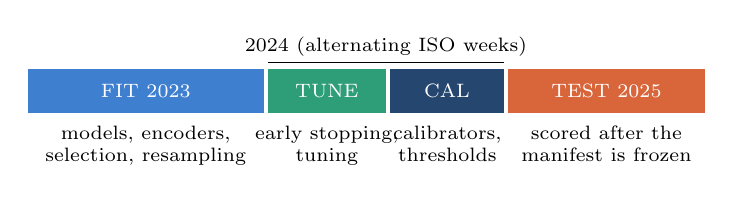
\begin{tikzpicture}[font=\scriptsize]
  \def\h{0.55}
  \fill[fitc]  (0,0)     rectangle (3.0,\h)  node[midway,white] {FIT 2023};
  \fill[tunec] (3.05,0)  rectangle (4.55,\h) node[midway,white] {TUNE};
  \fill[calc]  (4.6,0)   rectangle (6.05,\h) node[midway,white] {CAL};
  \fill[testc] (6.1,0)   rectangle (8.6,\h)  node[midway,white] {TEST 2025};
  \draw[thin] (3.05,\h+0.08) -- (6.05,\h+0.08);
  \node[above] at (4.55,\h+0.04) {2024 (alternating ISO weeks)};
  \node[align=center, below] at (1.5,-0.05) {models, encoders,\\ selection, resampling};
  \node[align=center, below] at (3.8,-0.05) {early stopping,\\ tuning};
  \node[align=center, below] at (5.33,-0.05) {calibrators,\\ thresholds};
  \node[align=center, below] at (7.35,-0.05) {scored after the\\ manifest is frozen};
\end{tikzpicture}
\caption{Temporal evaluation design. Final models are refitted on FIT+TUNE; CAL is reserved for calibration, thresholds and model selection.}
\label{fig:design}
\end{figure}

\subsection{Feature Sets (Factor FE)}

\textbf{F0} (168 features) is the raw set: 24 collision-level fields, 134 vehicle code counts, six minimum, mean and maximum summaries, and four pedestrian fields. \textbf{F1full} (244) adds 76 engineered features: temporal (cyclic hour and month, night, weekend, bank holiday), environmental (dark and unlit, poor weather, wet or icy surface), road (high speed, rural single carriageway at 60~mph or more, junction complexity), vehicle mix (vulnerable road user (VRU) involved, lightest and heaviest vehicle mass class, mass mismatch, and the relative heading of two vehicles computed from their compass directions), driver (young or older driver, age range), interaction terms, and out-of-fold $m$-estimate target encodings ($m=50$) of district, police force and a 5~km grid cell. \textbf{F1} (117) is the subset left after three selection steps on FIT rows: dropping near-constant features (one value in more than 99.5\% of rows; 35 dropped), dropping one feature of each pair with absolute Spearman correlation or Cram\'er's $V$ above 0.95 (25 dropped), and keeping features whose LightGBM permutation importance, measured as the drop in PR-AUC, was positive in at least three of four leave-one-quarter-out folds of 2023 (67 dropped).

\subsection{Cost-Sensitive Learning (Factor CS)}

Four strategies were applied to training rows only: \textit{none} (the natural ratio of about 3:1); \textit{weight}, in which each severe row receives weight $w=n_{-}/n_{+}$ computed on the training partition and not tuned ($w=3.18$ on FIT during tuning and $117{,}857/37{,}642=3.13$ on FIT+TUNE for the refit); \textit{rus}, random undersampling of slight collisions to 1:1; and \textit{smotenc}, SMOTE-NC~\cite{chawla2002smote} oversampling to 1:1 for logistic regression, random forest and LightGBM. Before SMOTE-NC, numeric features were median-imputed and standardised for the neighbour search, and integer-valued features were rounded after interpolation.

Let $p(x)=P(y=1\mid x)$. At the population optimum of the weighted log-loss, the score $p_w(x)$ satisfies
\begin{equation}
\frac{p_w(x)}{1-p_w(x)} = w\,\frac{p(x)}{1-p(x)},
\label{eq:odds}
\end{equation}
which follows from setting the derivative of $-wp\log q-(1-p)\log(1-q)$ with respect to $q$ to zero. Under this idealisation, a threshold of 0.5 on $p_w$ corresponds to $p\ge 1/(1+w)\approx 0.242$, the logit is shifted by $\ln w\approx 1.14$, and the ranking is unchanged. Separately tuned, regularised models need not follow (\ref{eq:odds}) exactly, so Section~\ref{sec:rq2} checks it against the fitted models.

\subsection{Calibration and Decision Thresholds (Factor CAL)}

Calibrators were fitted on the CAL predictions of each model. The Platt-style calibrator fits an unpenalised logistic regression on the logit of the model score, clipped to $[10^{-6},\,1-10^{-6}]$,
\begin{equation}
\hat p = \sigma\big(a\,\mathrm{logit}(p) + b\big),
\label{eq:platt}
\end{equation}
following Platt~\cite{platt1999probabilistic}. Isotonic regression~\cite{zadrozny2002transforming} fits a monotone non-decreasing map from $p$ to the observed rate. The method with the lower five-fold cross-fitted Brier score on CAL was chosen and refitted on all of CAL. Thresholds, by contrast, were optimised directly on the CAL labels, so only their 2025 performance is reported. We report the Brier score and an ECE computed over up to $B=15$ quantile bins (duplicate bin edges merged),
\begin{equation}
\mathrm{ECE} = \sum_{b=1}^{B} \frac{n_b}{n}\,\big|\bar y_b - \bar p_b\big|.
\label{eq:ece}
\end{equation}
A collision is flagged when $\hat p \ge t$. Five thresholds were fixed on CAL: the default $t=0.5$; $t^{*}$, which maximises $F_2 = 5PR/(4P+R)$; the most precise threshold with recall of at least 0.80; the threshold that minimises the empirical cost on CAL; and the Bayes threshold for an assumed cost of 5 for a missed severe collision and 1 for a false alarm,
\begin{equation}
t_{\mathrm{cost}} = \frac{c_{\mathrm{FP}}}{c_{\mathrm{FP}}+c_{\mathrm{FN}}} = \frac{1}{6}, \qquad
C = \frac{c_{\mathrm{FN}}\,\mathrm{FN} + c_{\mathrm{FP}}\,\mathrm{FP}}{n}.
\label{eq:cost}
\end{equation}
$C$ is the expected cost per collision. The Bayes threshold needs no search but is valid only for calibrated scores. The 5:1 ratio is our assumption, not an official figure.

%% ======================================================================
\section{Experimental Setup}

\subsection{Models and Tuning}

We used logistic regression (L2, one-hot encoding with rare levels pooled, median imputation with missing indicators), a decision tree and a random forest from scikit-learn (ordinal-coded categories), and XGBoost~\cite{chen2016xgboost}, LightGBM~\cite{ke2017lightgbm} and CatBoost~\cite{prokhorenkova2018catboost} with their native categorical handling. Each cell of the ablation had its own Optuna TPE study~\cite{akiba2019optuna} (seed 42) that maximised PR-AUC on TUNE at the natural prevalence, an objective that does not depend on a threshold. Budgets were 30 trials for the decision tree, XGBoost and LightGBM, 20 for CatBoost, and 15 for logistic regression, random forest and all SMOTE-NC cells, so LightGBM with SMOTE-NC received half the budget of the other LightGBM cells. Boosters stopped early on TUNE log-loss. Each refit was repeated with seeds 0, 1 and 2. XGBoost and CatBoost ran on an NVIDIA RTX A5000 GPU and the other models on CPU, using Python 3.12, scikit-learn 1.9, XGBoost 3.0.5, LightGBM 4.7, CatBoost 1.2 and SHAP 0.54.

\subsection{Ablation Matrix}

The factorial core \{F0, F1\} $\times$ \{none, weight, rus\} $\times$ six models gives 36 cells. Six SMOTE-NC cells, two F1full cells (logistic regression and LightGBM) and four sensitivity cells bring the total to 48 cells, or 144 refitted binary models. Each was scored raw and with both calibrators at the five thresholds.

\subsection{Statistical Analysis}

PR-AUC is computed as average precision. All 2025 comparisons are paired, because both arms score the same collisions, and use the seed-0 models. For each contrast we report the difference with a 95\% stratified percentile bootstrap interval (2,000 resamples) and a two-sided bootstrap $p$-value, together with DeLong's test for ROC-AUC~\cite{delong1988comparing} and McNemar's test on the paired decisions~\cite{mcnemar1947note}. One primary contrast per research question and model family (18 in total) was written into the manifest before 2025 was scored and Holm-corrected~\cite{holm1979simple}: $\Delta$PR-AUC of F1 versus F0 with no CS (RQ1); $\Delta F_2$ of weight versus none on F0, each at its own CAL-chosen $t^{*}$ (RQ2); and $\Delta$Brier of the CAL-chosen calibrator versus raw scores on F1 with the CAL-best strategy (RQ3). All other contrasts are exploratory. Within each model family, the strategy carried forward was the one with the highest calibrated $F_2$ on CAL. The final model was the cell with the highest mean raw PR-AUC on CAL; ties within 0.002 went to the lower calibrated Brier score and then to the simpler model. Because PR-AUC depends on prevalence~\cite{saito2015precision}, we also give its no-skill value (0.262 on 2025).

%% ======================================================================
\section{Results and Discussion}

Tables~\ref{tab:main} and~\ref{tab:ops} and Fig.~\ref{fig:prauc} report means over three seeds; for the configurations in Table~\ref{tab:main} the standard deviation of PR-AUC across seeds was at most 0.001. Contrasts (Table~\ref{tab:primary}), Figs.~\ref{fig:cscal} and~\ref{fig:threshold}, subgroup results and sensitivity analyses use the seed-0 models. Bracketed intervals are unadjusted 95\% bootstrap intervals.

\subsection{Overall Performance}

Table~\ref{tab:main} lists, for each model family, the F1 configuration with the CAL-chosen imbalance strategy. The three boosters are within 0.004 PR-AUC of each other, and the best of them is ahead of random forest by 0.013, logistic regression by 0.023 and the decision tree by 0.046. The final model, chosen on CAL by the rule above, was LightGBM with the F1full features and no cost-sensitive learning. On 2025 it reached a PR-AUC of 0.496 (1.9 times the no-skill value), an ROC-AUC of 0.730, a Brier score of 0.1675 and an ECE of 0.009. Both ranking metrics are higher than the values reported for STATS19 by Le~\cite{le2026ksi} and Alhawarat \textit{et al.}~\cite{alhawarat2026calibrated}, but the years, splits, feature sets and possibly the unit of analysis differ, so the comparison is only indicative. At $t^{*}$ the models flagged between 72\% and 81\% of collisions and reached $F_2$ of 0.660 to 0.668, against 0.640 for flagging every collision. Fig.~\ref{fig:prauc} shows PR-AUC for the main configurations.

\begin{table}[t]
\centering
\caption{F1 configuration with the CAL-chosen imbalance strategy (CS) per model family on 2025: Platt calibration, $F_2$-optimal threshold frozen on CAL, mean of three seeds. Bold marks the best unrounded PR-AUC, ROC-AUC, Brier score and $F_2$.}
\label{tab:main}
\setlength{\tabcolsep}{2.4pt}
\begin{tabular}{@{}llcccccc@{}}
\toprule
Model & CS & PR-AUC & ROC-AUC & Brier & ECE & Recall & $F_2$ \\
\midrule
LR & rus & 0.473 & 0.715 & 0.171 & 0.010 & 0.904 & 0.663 \\
DT & none & 0.451 & 0.700 & 0.174 & 0.010 & 0.936 & 0.660 \\
RF & weight & 0.484 & 0.724 & 0.169 & 0.009 & 0.918 & 0.666 \\
XGBoost & none & \textbf{0.497} & \textbf{0.731} & \textbf{0.167} & 0.009 & 0.911 & \textbf{0.668} \\
LightGBM & none & 0.496 & 0.731 & 0.167 & 0.010 & 0.903 & 0.668 \\
CatBoost & weight & 0.493 & 0.728 & 0.168 & 0.009 & 0.917 & 0.667 \\
\bottomrule
\end{tabular}
\end{table}

\begin{figure}[t]
\centering
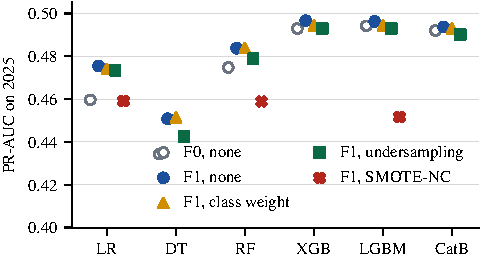
\includegraphics[width=\columnwidth]{figures/fig_prauc.pdf}
\caption{PR-AUC (average precision) on 2025 by model family for F0 without CS and for F1 under each imbalance strategy (raw scores, mean of three seeds). The no-skill value is 0.262. SMOTE-NC was run for LR, RF and LightGBM only.}
\label{fig:prauc}
\end{figure}

\subsection{RQ1: Feature Engineering}

The estimated gain from F1 over F0 varied by model family (Table~\ref{tab:primary}). It was largest for the decision tree (+0.0165), logistic regression (+0.0157) and random forest (+0.0089), and smaller but still significant after Holm correction for XGBoost (+0.0037). For LightGBM (+0.0014) and CatBoost (+0.0019) no significant gain was detected; CatBoost's unadjusted interval excludes zero, but its adjusted $p$ is 0.22. The small gains for the boosters suggest that they already extract much of the information in the engineered features from the raw codes. The F1full cells separate engineering from selection for two families: relative to F0, the engineered set without selection gained +0.018 for logistic regression and +0.0013 for LightGBM, while selection then removed 52\% of the columns with no detectable PR-AUC change for LightGBM and a loss of 0.0024 for logistic regression.

\begin{table*}[t]
\centering
\caption{Primary contrasts on 2025, seed-0 models. Brackets are unadjusted 95\% percentile bootstrap intervals; $p$ values are Holm-adjusted over the 18 primary tests (smallest attainable value 0.018). Bold: significant after adjustment.}
\label{tab:primary}
\setlength{\tabcolsep}{4pt}
\begin{tabular}{@{}lccc@{}}
\toprule
Model & RQ1: $\Delta$PR-AUC, F1 $-$ F0 & RQ2: $\Delta F_2$ at own $t^{*}$, weight $-$ none (F0) & RQ3: $\Delta$Brier, calibrated $-$ raw \\
\midrule
Logistic regression & \textbf{+0.0157} [+0.0131, +0.0183], $p=0.018$ & +0.0003 [$-$0.0003, +0.0009], $p=1.00$ & \textbf{$-$0.0443} [$-$0.0449, $-$0.0438], $p=0.018$ \\
Decision tree & \textbf{+0.0165} [+0.0125, +0.0206], $p=0.018$ & $-$0.0002 [$-$0.0021, +0.0020], $p=1.00$ & \textbf{$-$0.00036} [$-$0.00043, $-$0.00028], $p=0.018$ \\
Random forest & \textbf{+0.0089} [+0.0067, +0.0111], $p=0.018$ & +0.0009 [$-$0.0004, +0.0022], $p=0.87$ & \textbf{$-$0.0376} [$-$0.0380, $-$0.0371], $p=0.018$ \\
XGBoost & \textbf{+0.0037} [+0.0019, +0.0056], $p=0.018$ & +0.0004 [$-$0.0006, +0.0014], $p=1.00$ & \textbf{$-$0.00012} [$-$0.00014, $-$0.00011], $p=0.018$ \\
LightGBM & +0.0014 [$-$0.0001, +0.0029], $p=0.55$ & $-$0.0003 [$-$0.0014, +0.0008], $p=1.00$ & \textbf{$-$0.00011} [$-$0.00012, $-$0.00009], $p=0.018$ \\
CatBoost & +0.0019 [+0.0003, +0.0036], $p=0.22$ & +0.0006 [$-$0.0006, +0.0019], $p=1.00$ & \textbf{$-$0.0412} [$-$0.0418, $-$0.0407], $p=0.018$ \\
\bottomrule
\end{tabular}
\end{table*}

\subsection{RQ2: Cost-Sensitive Learning}
\label{sec:rq2}

The answer to RQ2 depends on the threshold. At 0.5, class weighting raised recall on F0 by +0.47 to +0.52 for every model; for LightGBM recall rose from 0.21 to 0.68 [+0.466, +0.478]. With each arm at its own $t^{*}$ chosen on CAL, none of the six primary contrasts was significant: the differences lay between $-0.0003$ and $+0.0009$, and every adjusted $p$ was at least 0.87. This is an absence of evidence for a gain, not a test of equivalence. On the threshold-free PR-AUC, weighting and undersampling changed results by between +0.001 and $-$0.021. SMOTE-NC lowered PR-AUC by 0.016 to 0.079 and $F_2$ by 0.005 to 0.009 in all six cells where it was used. A possible reason, which we did not test, is that interpolation creates records that police never report, for example a speed limit between the legal 30 and 60~mph values. The SMOTE-NC pipeline also differs in imputation and, for LightGBM, in tuning budget, so the result applies to the pipeline as a whole.

Equation (\ref{eq:odds}) suggests comparing the weighted model at $t=0.5$ with the unweighted model at $1/(1+w)=0.242$. Fig.~\ref{fig:cscal}(a) does this for LightGBM on F1. The weighted model at 0.5 had recall 0.663, precision 0.416 and flagged 41.8\% of collisions; the unweighted model at 0.242 had recall 0.684, precision 0.409 and flagged 43.9\%. The two operating points differ by about two points of recall and one point of precision. Weighting also raised the mean predicted risk from 0.249 to 0.449, against an observed rate of 0.262. On this data, then, most of the effect of class weighting at 0.5 can be reproduced by lowering the threshold of an unweighted model.

\begin{figure*}[t]
\centering
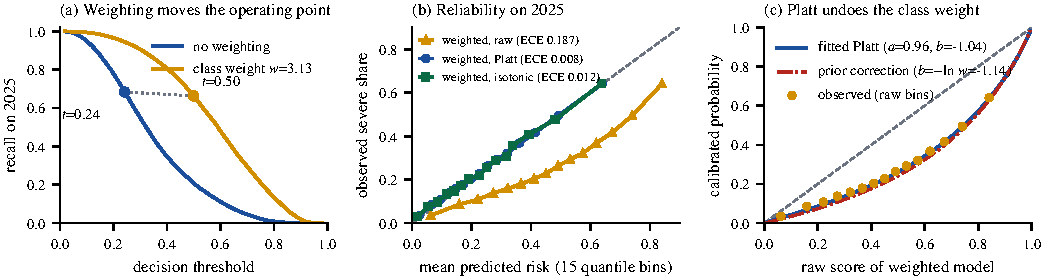
\includegraphics[width=\textwidth]{figures/fig_cs_cal.pdf}
\caption{LightGBM on F1, 2025, seed 0. (a) Recall against threshold with and without class weighting; the dotted segment joins the weighted model at 0.5 and the unweighted model at $1/(1+w)$. (b) Reliability of the weighted model before and after calibration on CAL. (c) Fitted Platt map, the prior correction $\sigma(\mathrm{logit}\,p - \ln w)$ implied by (\ref{eq:odds}), and the observed rates of the raw-score bins.}
\label{fig:cscal}
\end{figure*}

\subsection{RQ3: Calibration}

Calibration gave its largest improvements after weighting or undersampling. In those cells the raw scores overestimated risk, with ECE between 0.19 and 0.23 and Brier scores between 0.21 and 0.24. Calibrators fitted on CAL reduced the Brier score on 2025 by 0.038 to 0.044 in the primary tests for logistic regression, random forest and CatBoost, and ECE by 0.18 to 0.19. For the weighted LightGBM (Fig.~\ref{fig:cscal}(b)), ECE fell from 0.187 to 0.008 with Platt scaling and to 0.012 with isotonic regression. Boosters trained on the natural class balance were already close to calibrated (ECE about 0.01), and calibration improved their Brier score by only about 0.0001, which was nevertheless significant.

The Platt fit for the weighted LightGBM was $a=0.96$ and $b=-1.04$ (Fig.~\ref{fig:cscal}(c)). Equation (\ref{eq:odds}) gives $a=1$ and $b=-\ln w=-1.14$ for the ideal case, so the correction learned from CAL is close to the one implied by the class weight. For the final unweighted model the fit was $a=1.01$ and $b=0.05$, near the identity. Platt scaling had the lower cross-fitted Brier score for every configuration in Table~\ref{tab:main}, and on 2025 the three-seed mean Brier scores of the two calibrators differed by at most 0.00014. For the final model isotonic regression also lowered PR-AUC slightly (0.4875 against 0.4960), because it maps ranges of scores to the same value.

\subsection{Threshold Selection and Expected Cost}

Threshold selection changed detection and cost far more than any other factor (Table~\ref{tab:ops}, Fig.~\ref{fig:threshold}). At 0.5 the final model found 20.9\% of severe collisions. At the Bayes threshold of 1/6 on Platt-calibrated scores it found 85.6\% at a precision of 34.7\% and flagged 64.8\% of collisions. Expected cost fell from 1.072 to 0.612 per collision ($-43\%$), which is also 17\% below the cost of flagging every collision (0.738). At 1/6, calibration lowered the mean cost of this model only from 0.613 (raw scores) to 0.612. Calibration matters for the models trained with weights or undersampling. For the weighted LightGBM, the three-seed mean cost at 1/6 was 0.664 with raw scores and 0.614 after Platt scaling, and the gap was 0.05 to 0.07 for the other weighted or undersampled cells in Table~\ref{tab:main}. On the seed-0 calibrated scores, the threshold that minimised cost on 2025 was 0.167, essentially equal to 1/6. The recall-constrained threshold chosen on CAL gave a recall of 0.797 on 2025, just below its 0.80 target.

\begin{table}[t]
\centering
\caption{Operating points of the final model on 2025 (mean of three seeds). Cost uses $c_{\mathrm{FN}}=5$, $c_{\mathrm{FP}}=1$.}
\label{tab:ops}
\setlength{\tabcolsep}{3pt}
\begin{tabular}{@{}lccccc@{}}
\toprule
Scores, threshold & $t$ & Recall & Prec. & Flagged & Cost \\
\midrule
Raw, $t=0.5$ & 0.500 & 0.209 & 0.613 & 9.0\% & 1.072 \\
Platt, $t=0.5$ & 0.500 & 0.223 & 0.605 & 9.7\% & 1.057 \\
Platt, recall $\ge 0.80$ on CAL & 0.198 & 0.797 & 0.370 & 56.6\% & 0.623 \\
Raw, $t=1/6$ & 0.167 & 0.849 & 0.349 & 63.8\% & 0.613 \\
Platt, $t=1/6$ & 0.167 & 0.856 & 0.347 & 64.8\% & 0.612 \\
Platt, $F_2$-optimal $t^{*}$ & 0.138 & 0.904 & 0.327 & 72.5\% & 0.615 \\
Flag every collision & -- & 1.000 & 0.262 & 100\% & 0.738 \\
\bottomrule
\end{tabular}
\end{table}

\begin{figure}[t]
\centering
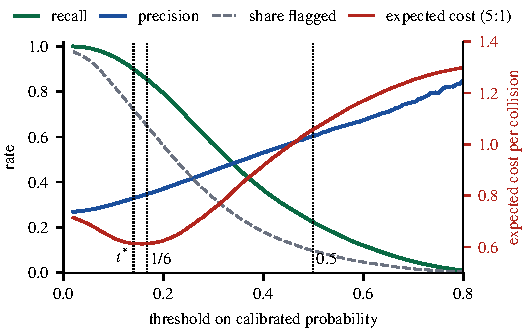
\includegraphics[width=\columnwidth]{figures/fig_threshold.pdf}
\caption{Final model on 2025 (Platt-calibrated, seed 0): recall, precision and share flagged (left axis) and expected cost at a 5:1 cost ratio (right axis). Dotted lines mark thresholds frozen on CAL.}
\label{fig:threshold}
\end{figure}

\subsection{Temporal Stability and Subgroups}

The 2025 year contains a known shift. Injury-based recording systems, which classify more injuries as serious, covered 53.7\% of collisions in 2023, 58.8\% in 2024 and 86.5\% in 2025~\cite{dft2026stats19}. Averaged over all 48 cells, ROC-AUC fell by 0.013 from CAL to 2025, and the ranking of the cells by PR-AUC was stable (Spearman correlation 0.986). The calibrated mean prediction of the final model was 25.6\% against an observed 26.2\%. The overall figures hide larger differences between subgroups. The final model ranked collisions better within officer-judged forces (ROC-AUC 0.773) than within injury-based forces (0.723). At $t^{*}$ its recall was 0.93 for collisions attended by the police and 0.64 for self-reported ones, and its ECE was 0.022 for attended, 0.059 for non-attended and 0.025 for self-reported collisions.

\subsection{Explanations}

Exact TreeSHAP attributions~\cite{lundberg2017unified,lundberg2020local} on the log-odds scale were computed for the final model on 20,000 collisions each from CAL and 2025. The ranking of mean absolute SHAP values was almost the same in both years (Spearman $\rho=0.9995$, Fig.~\ref{fig:shap}). Among the leading features are the involvement of a vulnerable road user, the speed limit, the mass class of the lightest vehicle and the relative heading of two vehicles; head-on headings raise the predicted risk and same-direction movements lower it. Several high-ranking features describe the record rather than the crash: police force, the number of drivers of unknown age and counts of missing values for driver deprivation decile and left-hand drive. Higher values of the missing-data features lower the predicted risk, and in the data missingness is associated with lower recorded severity. These are model attributions, not causal effects, but part of the signal clearly reflects recording practice.

\begin{figure}[t]
\centering
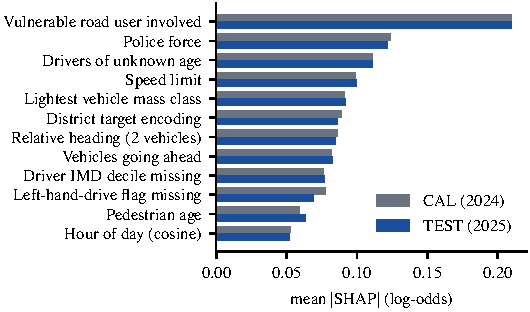
\includegraphics[width=\columnwidth]{figures/fig_shap.pdf}
\caption{Mean absolute TreeSHAP value (log-odds) of the twelve most important features of the final model on CAL (2024) and TEST (2025), 20,000 collisions each.}
\label{fig:shap}
\end{figure}

\subsection{Limitations}

The availability rule is an assumption about retrospective records; we did not verify which fields are known when a collision is first reported, and the pedestrian fields describe an injured pedestrian. STATS19 covers only injury collisions reported to the police, and the severity label changed over time as injury-based recording spread. Target encoding was not nested within the quarter-based selection folds, so the selection importances may be optimistic; CAL and 2025 labels were not used in this step, and the effect on the selected features was not measured. The bootstrap intervals treat collisions as independent and condition on the seed-0 model, so they do not include clustering by week or force or training variability. Tuning budgets were 15 to 30 trials per cell and were not equal across strategies for LightGBM.

%% ======================================================================
\section{Ablation and Sensitivity Studies}
\label{sec:sens}

Table~\ref{tab:sens} gives four sensitivity analyses with XGBoost on F1 without CS, each compared with the primary XGBoost model, and one three-class LightGBM model. Adding the five held-out crash-mechanics fields (skidding, objects hit, leaving the carriageway, first point of impact) increased PR-AUC by 0.012. These fields describe the impact itself, which is why the main model excludes them. Replacing all remaining missing values by the training median or mode (S2) cost 0.003, although explicit missing-value count features were kept. S2 and S5 reuse the F1 selection rather than repeating it. Dropping police force and recording-system variables (S3) cost 0.002; district encodings and other correlated features may still carry information about recording practice. Removing the pedestrian fields together with the VRU features that use them (S5) cost 0.019, giving a PR-AUC of 0.477 for that model. Separating fatal from serious collisions was much harder: a class-balanced three-class LightGBM, trained once (seed 0) with the binary model's hyper-parameters, reached a macro-F1 of 0.450 and a fatal recall of 0.45 at a precision of 0.10.

\begin{table}[t]
\centering
\caption{Sensitivity analyses on 2025 (S1--S3, S5: XGBoost, F1, no CS, seed 0, paired with the primary XGBoost model)}
\label{tab:sens}
\setlength{\tabcolsep}{3pt}
\begin{tabular}{@{}lcc@{}}
\toprule
Analysis & $\Delta$PR-AUC [95\% CI] & $\Delta$ROC-AUC \\
\midrule
S1: + crash mechanics & +0.0117 [+0.010, +0.014] & +0.0078 \\
S2: median/mode imputation & $-$0.0030 [$-$0.004, $-$0.002] & $-$0.0016 \\
S3: no force/recording variables & $-$0.0023 [$-$0.003, $-$0.001] & $-$0.0013 \\
S5: no pedestrian/VRU fields & $-$0.0192 [$-$0.022, $-$0.017] & $-$0.0112 \\
\midrule
S4: three classes (LightGBM) & \multicolumn{2}{l}{macro-F1 0.450; fatal recall 0.45,} \\
 & \multicolumn{2}{l}{fatal precision 0.10} \\
\bottomrule
\end{tabular}
\end{table}

%% ======================================================================
\section{Conclusion and Future Work}

Engineered features improved ranking most for logistic regression and the single tree, with smaller gains for the boosters. Class weighting and undersampling raised recall at the default threshold, but in the six primary comparisons no significant $F_2$ benefit from class weighting was detected once each arm used its CAL-selected threshold, and SMOTE-NC lowered performance in every configuration where it was tested. Calibration was needed after weighting or undersampling, and the Platt correction it learned was close to the one implied by the class weight. The largest change came from the threshold: under an assumed 5:1 cost ratio, the threshold 1/6 raised recall from 0.21 to 0.86 and lowered expected cost by 43\%. For STATS19 data, a reasonable starting point is a gradient-boosting model with engineered features, trained on the natural class balance, calibrated on recent held-out data and thresholded according to the chosen cost ratio, with calibration rechecked when police forces change their recording systems. Future work should add road-geometry and traffic-volume data, test transfer between police forces, re-estimate the models once injury-based recording is universal, and study fatal collisions with their own cost structure.

\bibliographystyle{IEEEtran}
\bibliography{refs}

\end{document}
